% A model trained on biased records learns where people looked.
% ---------------------------------------------------------------------------
% style.tex --- shared preamble for every figure in book/figures/tikz/
%
% One style for all figures: Latin Modern, thin black lines, a light grey
% fill, and one accent colour used only to mark what is untrusted or wrong.
% Build with scripts/build_figures.sh; see book/figures/README.md.
% ---------------------------------------------------------------------------
\documentclass[tikz,border=6pt]{standalone}
\usepackage[T1]{fontenc}
\usepackage{lmodern}
\usetikzlibrary{arrows.meta,positioning,shapes.geometric,calc,fit,backgrounds}

\hyphenpenalty=10000   % short lines in boxes: ragged, never hyphenated

\definecolor{lightgrey}{gray}{0.92}
\definecolor{accent}{HTML}{9B2D20}

\tikzset{
  every picture/.style={
    line width=0.6pt,
    font=\small,
    >={Stealth[length=5pt,width=4pt]},
    node distance=14pt and 24pt,
  },
  % shapes
  box/.style={draw, rectangle, inner xsep=8pt, inner ysep=5pt,
              minimum height=22pt, align=center},
  grey/.style={box, fill=lightgrey},
  rounded/.style={box, rounded corners=9pt},
  decision/.style={draw, diamond, aspect=2.4, inner sep=1.5pt, align=center},
  group/.style={draw, dashed, rounded corners=5pt, inner sep=7pt},
  % text
  tag/.style={font=\footnotesize, align=center, inner sep=2pt},
  note/.style={font=\footnotesize\itshape, align=center, inner sep=2pt},
  code/.style={font=\small\ttfamily},
  codetag/.style={font=\footnotesize\ttfamily, align=center, inner sep=2pt},
  title/.style={font=\small\scshape, align=center, inner sep=2pt},
  % lines
  arrow/.style={->},
  back/.style={->, dashed},
  thin/.style={line width=0.4pt, gray},
  % the one accent, for what is untrusted, wrong or missing
  bad/.style={accent},
  badbox/.style={box, draw=accent, text=accent},
}

\begin{document}
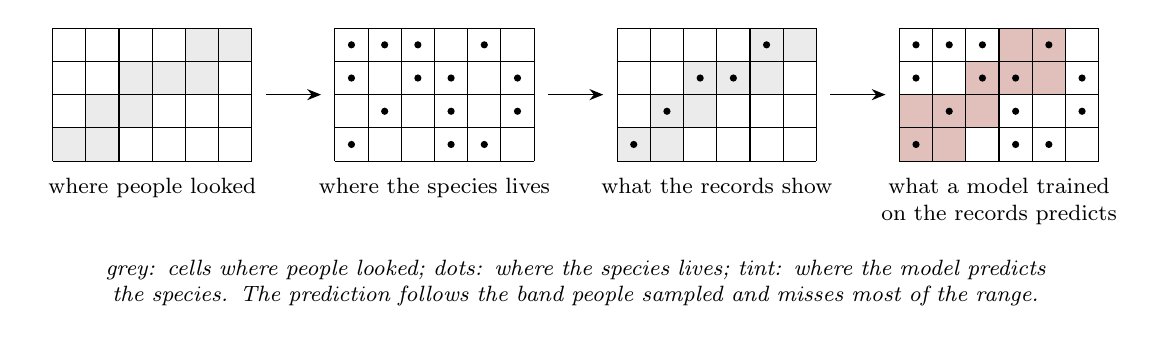
\begin{tikzpicture}[c/.store in=\cell, c=12pt]
  % sampled cells (A, C), occurrences (B, C, D), predicted presence (D)
  \def\sampled{0/0,1/0,1/1,2/1,2/2,3/2,4/2,4/3,5/3}
  \def\lives{0/0,1/1,2/2,3/2,4/3,0/3,1/3,3/0,4/0,5/1,2/3,5/2,0/2,3/1}
  \def\records{0/0,1/1,2/2,3/2,4/3}
  \def\predicted{0/0,1/0,0/1,1/1,2/1,2/2,3/2,4/2,3/3,4/3}
  % panel A: where people looked
  \begin{scope}
    \foreach \i/\j in \sampled
      \fill[lightgrey] (\i*\cell,\j*\cell) rectangle ++(\cell,\cell);
    \draw[thin, black] (0,0) grid[step=\cell] (6*\cell,4*\cell);
    \node[tag, text width=86pt, anchor=north] at (3*\cell,-4pt) {where people looked};
  \end{scope}
  % panel B: where the species lives
  \begin{scope}[shift={(102pt,0)}]
    \foreach \i/\j in \lives
      \fill (\i*\cell+\cell/2,\j*\cell+\cell/2) circle (1.3pt);
    \draw[thin, black] (0,0) grid[step=\cell] (6*\cell,4*\cell);
    \node[tag, text width=86pt, anchor=north] at (3*\cell,-4pt) {where the species lives};
  \end{scope}
  % panel C: what the records show
  \begin{scope}[shift={(204pt,0)}]
    \foreach \i/\j in \sampled
      \fill[lightgrey] (\i*\cell,\j*\cell) rectangle ++(\cell,\cell);
    \foreach \i/\j in \records
      \fill (\i*\cell+\cell/2,\j*\cell+\cell/2) circle (1.3pt);
    \draw[thin, black] (0,0) grid[step=\cell] (6*\cell,4*\cell);
    \node[tag, text width=86pt, anchor=north] at (3*\cell,-4pt) {what the records show};
  \end{scope}
  % panel D: what a model trained on the records predicts
  \begin{scope}[shift={(306pt,0)}]
    \foreach \i/\j in \predicted
      \fill[accent!30] (\i*\cell,\j*\cell) rectangle ++(\cell,\cell);
    \foreach \i/\j in \lives
      \fill (\i*\cell+\cell/2,\j*\cell+\cell/2) circle (1.3pt);
    \draw[thin, black] (0,0) grid[step=\cell] (6*\cell,4*\cell);
    \node[tag, text width=86pt, anchor=north] at (3*\cell,-4pt) {what a model trained on the records predicts};
  \end{scope}
  \draw[->] (77pt,2*\cell) -- (97pt,2*\cell);
  \draw[->] (179pt,2*\cell) -- (199pt,2*\cell);
  \draw[->] (281pt,2*\cell) -- (301pt,2*\cell);
  \node[note, text width=370pt] at (189pt,-44pt)
    {grey: cells where people looked; dots: where the species lives; tint: where
     the model predicts the species. The prediction follows the band people
     sampled and misses most of the range.};
\end{tikzpicture}
\end{document}
